%% Hlavní soubor. Zde se definují základní parametry a odkazuje se na ostatní části. %%%

%% Verze pro jednostranný tisk:
% Okraje: levý 40mm, pravý 25mm, horní a dolní 25mm
% (ale pozor, LaTeX si sám přidává 1in)
\documentclass[12pt,a4paper]{report}
\setlength\textwidth{145mm}
\setlength\textheight{247mm}
\setlength\oddsidemargin{15mm}
\setlength\evensidemargin{15mm}
\setlength\topmargin{0mm}
\setlength\headsep{0mm}
\setlength\headheight{0mm}
% \openright zařídí, aby následující text začínal na pravé straně knihy
\let\openright=\clearpage

%% Pokud tiskneme oboustranně:
% \documentclass[12pt,a4paper,twoside,openright]{report}
% \setlength\textwidth{145mm}
% \setlength\textheight{247mm}
% \setlength\oddsidemargin{15mm}
% \setlength\evensidemargin{0mm}
% \setlength\topmargin{0mm}
% \setlength\headsep{0mm}
% \setlength\headheight{0mm}
% \let\openright=\cleardoublepage

%% Pokud používáte csLaTeX (doporučeno):
\usepackage{czech}
%% Pokud nikoliv:
%\usepackage[czech]{babel}
%\usepackage[T1]{fontenc}

%% Použité kódování znaků: obvykle latin2, cp1250 nebo utf8:
\usepackage[utf8]{inputenc}

%% Ostatní balíčky
\usepackage{graphicx}
\usepackage{amsthm}
\usepackage{amsmath}
\usepackage{listings}
\usepackage{tikz}

%% Balíček hyperref, kterým jdou vyrábět klikací odkazy v PDF,
%% ale hlavně ho používáme k uložení metadat do PDF (včetně obsahu).
%% POZOR, nezapomeňte vyplnit jméno práce a autora.
\usepackage[ps2pdf,unicode]{hyperref}   % Musí být za všemi ostatními balíčky
\hypersetup{pdftitle=Nástroj pro porovnávání a vyhodnocování strojových překladů}
\hypersetup{pdfauthor=Ondřej Klejch}

%%% Drobné úpravy stylu

% Tato makra přesvědčují mírně ošklivým trikem LaTeX, aby hlavičky kapitol
% sázel příčetněji a nevynechával nad nimi spoustu místa. Směle ignorujte.
\makeatletter
\def\@makechapterhead#1{
  {\parindent \z@ \raggedright \normalfont
   \Huge\bfseries \thechapter. #1
   \par\nobreak
   \vskip 20\p@
}}
\def\@makeschapterhead#1{
  {\parindent \z@ \raggedright \normalfont
   \Huge\bfseries #1
   \par\nobreak
   \vskip 20\p@
}}
\makeatother

% Toto makro definuje kapitolu, která není očíslovaná, ale je uvedena v obsahu.
\def\chapwithtoc#1{
\chapter*{#1}
\addcontentsline{toc}{chapter}{#1}
}

\begin{document}

% Trochu volnější nastavení dělení slov, než je default.
\lefthyphenmin=2
\righthyphenmin=2

%%% Titulní strana práce

\pagestyle{empty}
\begin{center}

\large

Univerzita Karlova v Praze

\medskip

Matematicko-fyzikální fakulta

\vfill

{\bf\Large BAKALÁŘSKÁ PRÁCE}

\vfill

\centerline{\mbox{\includegraphics[width=60mm]{img/logo.eps}}}

\vfill
\vspace{5mm}

{\LARGE Ondřej Klejch}

\vspace{15mm}

% Název práce přesně podle zadání
{\LARGE\bfseries Nástroj pro porovnávání a vyhodnocování strojového překladu}

\vfill

% Název katedry nebo ústavu, kde byla práce oficiálně zadána
% (dle Organizační struktury MFF UK)
Název katedry nebo ústavu

\vfill

\begin{tabular}{rl}

Vedoucí bakalářské práce: & Mgr. Martin Popel \\
\noalign{\vspace{2mm}}
Studijní program: & Informatika  \\
\noalign{\vspace{2mm}}
Studijní obor: & Obecná informatika \\
\end{tabular}

\vfill

% Zde doplňte rok
Praha 2013

\end{center}

\newpage

%%% Následuje vevázaný list -- kopie podepsaného "Zadání bakalářské práce".
%%% Toto zadání NENÍ součástí elektronické verze práce, nescanovat.

%%% Na tomto místě mohou být napsána případná poděkování (vedoucímu práce,
%%% konzultantovi, tomu, kdo zapůjčil software, literaturu apod.)

\openright

\noindent
Poděkování.

\newpage

%%% Strana s čestným prohlášením k bakalářské práci

\vglue 0pt plus 1fill

\noindent
Prohlašuji, že jsem tuto bakalářskou práci vypracoval(a) samostatně a výhradně
s~použitím citovaných pramenů, literatury a dalších odborných zdrojů.

\medskip\noindent
Beru na~vědomí, že se na moji práci vztahují práva a povinnosti vyplývající
ze zákona č. 121/2000 Sb., autorského zákona v~platném znění, zejména skutečnost,
že Univerzita Karlova v Praze má právo na~uzavření licenční smlouvy o~užití této
práce jako školního díla podle §60 odst. 1 autorského zákona.

\vspace{10mm}

\hbox{\hbox to 0.5\hsize{%
V ........ dne ............
\hss}\hbox to 0.5\hsize{%
Podpis autora
\hss}}

\vspace{20mm}
\newpage

%%% Povinná informační strana bakalářské práce

\vbox to 0.5\vsize{
\setlength\parindent{0mm}
\setlength\parskip{5mm}

Název práce:
Nástroj pro porovnávání a vyhodnocování strojových překladů
% přesně dle zadání

Autor:
Ondřej Klejch

Ústav:
Ústav formální a aplikované lingvistiky

% dle Organizační struktury MFF UK

Vedoucí bakalářské práce:
Mgr. Martin Popel
% dle Organizační struktury MFF UK, případně plný název pracoviště mimo MFF UK

Abstrakt:
Tato bakalářská práce se zabývá vývojem nástroje pro porovnávání a vyhodnocování strojových překladů nazvaného MT-ComparEval.
Tento nástroj umožňuje organizovat překlady do skupin, aby je mohl vyhodnocovat proti různým referenčním překladům.
V tomto nástroji je možné porovnávat překlady na základě několika kriterií.
Mezi ně patří porovnání podle metrik strojových překladů počítaných pro celé dokumenty nebo jednotlivé věty,
  porovnání kvality překladů jednotlivých vět pomocí zvýraznění potvrzených, zlepšujících nebo zhoršujících n-gramů
  nebo souhrnu nejvíce zlepšujících či zhoršujících n-gramů v celém dokumentu.
MT-ComparEval také umožňuje uživatelské přizpůsobení pomocí doprogramování dalších metrik strojového překladu.


Klíčová slova:
porovnání překladů, vyhodnocování strojových překladačů, metriky strojových překladů
% 3 až 5 klíčových slov

\vss}\nobreak\vbox to 0.49\vsize{
\setlength\parindent{0mm}
\setlength\parskip{5mm}

Title:
Tool for Machine Translation Comparison and Evaluation
% přesný překlad názvu práce v angličtině

Author:
Ondřej Klejch

Department:
Institute of Formal and Applied Linguistics
% dle Organizační struktury MFF UK v angličtině

Supervisor:
Mgr. Martin Popel
% dle Organizační struktury MFF UK, případně plný název pracoviště
% mimo MFF UK v angličtině

Abstract:
% abstrakt v rozsahu 80-200 slov v angličtině; nejedná se však o překlad
% zadání bakalářské práce

Keywords:
% 3 až 5 klíčových slov v angličtině

\vss}

\newpage

%%% Strana s automaticky generovaným obsahem bakalářské práce. U matematických
%%% prací je přípustné, aby seznam tabulek a zkratek, existují-li, byl umístěn
%%% na začátku práce, místo na jejím konci.

\openright
\pagestyle{plain}
\setcounter{page}{1}
\tableofcontents

%%% Jednotlivé kapitoly práce jsou pro přehlednost uloženy v samostatných souborech
\chapwithtoc{Úvod}
Současný vývoj softwarových projektů probíhá v~krátkých iteracích,
  aby mohl pružně reagovat na změny v~zadání.
Stejně tak i vývoj strojových překladačů probíhá v~krátkých iteracích,
  aby bylo možné pravidelně ověřovat zlepšení nebo zhoršení kvality překladů.
Z~toho plyne potřeba vývojářů testovat změny,
  které provedli v~rámci iterace,
  která mohla trvat 30 sekund, hodinu, den nebo týden.
K~testování funkčnosti softwarových projektů lze použít různé sady testů -- od unit testů po akceptační testy.
Je možné stejným způsobem testovat i kvalitu strojových překladačů?

Je samozřejmé, 
  že vývojáři strojových překladačů testují svůj kód stejně jako ostatní vývojáři.
Pomocí těchto testů mohou zajistit,
  aby překladač fungoval,
  ale nemohou takto jednoduše zajistit kontrolu kvality překladů.
Kontrolu překladů může provádět sám vývojář,
  ale ztratí tím spoustu času a energie,
  kterou by mohl lépe využít při dalším vývoji.

Žádná kontrola kvality, kterou není možné automatizovat,
  vývojářům nepomůže zrychlit vývojový cyklus.
Proto je třeba,
  aby existoval způsob jak rychle a opakovaně kontrolovat kvalitu překladů.

Proto byly vynalezeny metriky strojového překladu,
  které umožňují rychle a opakovaně testovat překlady.
Tyto metriky se snaží hodnotit překlady tak,
  aby jejich výsledky co nejvíce odpovídaly lidskému hodnocení.

Avšak výsledek většiny metrik je pouhé jedno číslo.
Je třeba, aby vývojaři měli k~dispozici nástroje,
  pomocí kterých budou moci efektivně vyhodnocovat své překlady.
Pomocí takovýchto nástrojů si vývojáři mohou vyhodnotit,
  co způsobily změny, které provedli.

Vývojář by měl mít možnost překlady nejen vyhodnocovat,
  ale i porovnávat.
Porovnání dvou různých překladů může totiž vývojáři objasnit jevy,
  o~kterých nemusel vůbec vědět.
A~na základě takto získaných poznatků pak může vyvinout novou lepší verzi překladače.
A~po mnoha iteracích vývoje snad vyvine překladač,
  s~kterým bude moci být spokojený.

Na trhu existuje několik nástrojů,
  které umožňují vyhodnocovat překlady pomocí různých metrik
  nebo porovnávat překlady na základě různých kritérií.
Důležité je,
  aby mohl vývojář použít přístup,
  který mu vyhovuje.

Nástrojem,
  který umožňuje vývojářům efektivně porovnávat a vyhodnocovat překlady,
  se snaží být \mbox{MT-ComparEval}, 
  o~němž pojednává tato bakalářská práce.

\chapter{Motivace}
V této kapitole budou v krátkosti představeny všechny důvody,
  proč a jak byl vyvinut nástroj MT-ComparEval.
Všechny důvody pak budou více rozebrány v~následujících kapitolách.

\section{Experimenty a tasky}
Při vyhodnocování strojových překladů porovnání s referenčním překladem
  (dále budeme používat pouze reference).
Strojové překladače mohou být zaměřeny na různé domény textu (např. novinové články, beletrie apod.) 
  nebo na různé jazykové páry (např. z angličtiny do češtiny, z němčiny do češtiny apod.).
Aby uživatelé nástroje MT-ComparEval mohli snadno vyhodnocovat své strojové překladače na různých doménách nebo pro různé jazykové páry,
  mohou si vytořit různé \uv{experimenty},
  v rámci kterých mohou porovnávat své překlady s příslušnými referencemi.
Na Obrázku \ref{img:experiments} je vidět příklad vytvořených experimentů z různých domén a jazykových párů.
\begin{figure}
	\caption{Přehled vytvořených experimentů v nástroji MT-ComparEval}
	\label{img:experiments}
\end{figure}

V každém experimentu pak uživatel může vytvářet \uv{tasky},
  které později může vyhodnocovat a porovnávat.
Výpis tasků jednoho z experimentů je ukázán na Obrázku \ref{img:tasks}.
\begin{figure}
	\caption{Přehled vytvořených tasků v jednom z experimentů v nástroji MT-ComparEval}
	\label{img:tasks}
\end{figure}

O významu experimentů, tasků a jiných pojmů je možné se více dozvědět ve~\ref{chap:experiments}.~kapitole.


\section{Metriky strojového překladu}
Aby bylo možné jednotlivé překlady porovnávat,
  byly vynalezeny metriky 
V nástroji MT-ComparEval jsou metriky počítány na úrovni celých tasků 
  (na Obrázku \ref{img:compare_metrics_tasks} je vidět porovnání metrik dvou tásků)
  nebo na úrovni jednotlivých vět
  (Obrázek \ref{img:compare_metrics_sentences} ukazuje porovnání metrik pro dva různé překlady).
Metrikami strojových překladů se více zabývá \ref{chap:metrics}. kapitola.
V té budou představeny všechny metriky,
  které jsou použity v nástroji MT-ComparEval.

\begin{figure}
	\caption{Porovnání metrik dvou tasků v nástroji MT-ComparEval.}
	\label{img:compare_metrics_tasks}
\end{figure}

\begin{figure}
	\caption{Porovnání metrik dvou překladů v nástroji MT-ComparEval.}
	\label{img:compare_metrics_sentences}
\end{figure}


\section{Porovnávaní dvou strojových překladů}
Kvalitu strojových překladačů je možné vyhodnotit i porovnáním jednotlivých vět.
Nástroj MT-ComparEval umožňuje procházet věty seřazené podle metriky strojových překladů 
  a hledat v těchto větách rozdíly,
  které ovlivnily výsledné metriky.
Aby uživatelé mohli hledat rozdíly mezi větami,
  je možné zobrazit potvrzené n-gramy (n-gramy, které se nacházeji v referenci i strojovém překladu),
  zlepšující n-gramy (potvrzené n-gramy, které se nacházejí pouze v jednom z porovnávaných překladů)
  nebo zhoršující n-gramy (nepotvrzené n-gramy, které se nacházejí pouze v jednom z porovnávaných překladů).
Na Obrázku \ref{img:compare_sentences} je vidět porovnání dvou překladů se zvýrazněnými n-gramy.

Strojové překlady nemusejí být porovnávány pouze na základě strojových metrik,
  další informací,
  díky které je možné si udělat lepší představu o vlastnostech strojového překladače,
  jsou přehledy nejvíce zlepšujících a zhoršujících n-gramů v jednotlivých překladech.
Nástroj MT-ComparEval nabízí přehled nejvíce zlepšujících a zhoršujících n-gramů
  v jednotlivých překladech.
Takový přehled je možné vidět i na obrázku \ref{img:confirmed_ngrams}.

Přehledy zlepšujících i zhoršujicích n-gramů mohou byt použity k filtrování vět,
  aby si uživatel mohl snadno prohlédnout věty,
  ve kterých se dané n-gramy nacházejí.
Na Obrázku \ref{img:filtered_sentences} je vidět výpis vět vyfiltrovaných podle zlepšujícího n-gramu.


\begin{figure}
	\caption{
		Porovnání dvou překladů v nástroji MT-ComparEval.
		Pastelovými odstíny žluté a modré barvy jsou zvýrazněny potvrzené n-gramy,
		sytými odstíny žluté a modré barvy jsou zvýrazněny zlepšující n-gramy
		a červenou barvou jsou zvýrazněny zhoršující n-gramy.
	}
	\label{img:compare_sentences}
\end{figure}

\begin{figure}
	\caption{Přehled nejvíce zlepšujících n-gramů v jednotlivých překladech.}
	\label{img:confirmed_ngrams}
\end{figure}

\begin{figure}
	\caption{Výpis vět, v kterých se nachází zlepšující n-gram ??}
	\label{img:filtered_sentences}
\end{figure}

O algoritmech,
  které byly použity při porovnávání dvou překladů a hledání pozic potvrzených n-gramů,
  pojednává \ref{chap:compare}. kapitola.


\section{Automatizace a snadné použití}
Nástroj MT-ComparEval byl navržen tak,
  aby bylo možné jeho použití co nejvíce automatizovat.
Uživatelé tak nemusí ručne vytvářet každý task,
  ale mohou si napsat jednoduché skripty,
  pomocí nichž mohou vytvářet tasky automaticky při každém commitu, buildu,\dots

V \ref{chap:users}. kapitole je možné najít informace,
  jak se používá nástroj MT-ComparEval
  a jak je možné nasadit ho do vývojového procesu.

\section{Rozšiřitelnost}
Každý uživatel může preferovat různé metriky pro vyhodnocování strojových překladů.
V nástroji MT-ComparEval jsou předprogramovány pouze některé.
  avšak uživatel si může snadno doimplementovat svoje vlastní.

O tom, jak si uživatel může doprogramovat vlastní metriky nebo jak byl nástroj MT-ComparEval vyvinut,
  je možné se dočíst v \ref{chap:programmers}. kapitole.


\chapter{Názvosloví MT-ComparEval}
\label{chap:experiments}

Správné pochopení pojmů \textbf{experiment},\textbf{task}, \textbf{\mbox{n-gram}}, \dots je důležité k pochopení fungování celého nástroje MT-ComparEval.
Proto v této kapitole bude podrobněji vysvětleno,
  co tyto pojmy znamenají a jaké jsou mezi nimi vztahy.

\section{Experiment}
Uživatelé mohou chtít testovat své překladače na různých textových doménách různých délek
  nebo testovat své překladače pro různé jazykové páry.
Nástroj MT-ComparEval musí umožňovat vytvořit různá vyhodnocovací prostředí,
  ve kterých uživatelé mohou testovat své strojové překladače.
Takovéto testovací prostředí se v nástroji MT-ComparEval nazývá \textbf{experiment}.

Každý experiment obsahuje vlastní \textbf{zdroj} (věty, které mají být strojovým překladačem přeloženy) a
  \textbf{referenci} (člověkem přeložené věty, které budou později použity k vyhodnocování jednotlivých strojových překladačů).
Pomocí různých dvojic zdrojů a referencí mohou uživatelé vyhodnocovat strojové překladače na různých testovacích sadách,
  což se jim může hodit v případě,
  kdy se překladač na různých zdrojích chová různě.

\section{Task}
V rámci experimetu uživatelé mohou chtít porovnávat různé překlady zdrojových vět.
Ať už se jedná o různé verze jednoho strojového překladače nebo různé strojové překladače.
Aby mohl uživatel vyhodnocovat různé překlady,
  umožňuje nástroj MT-ComparEval nahrávat do experimentů tzv. \textbf{tasky}.
Každý task reprezentuje jednu verzi překladu zdrojových vět,
  která později může být porovnána s jinou verzí překladu.
V rámci této bakalářské práce budou strojové překlady nazývány zkráceně slovem \textbf{překlady}.

O vytváření experimentů a tasků i o dalších možnostech použití nástroje MT-ComparEval je možné se dozvědět v \ref{chap:users}. kapitole.

\section{N-gramy}
Při vysvětlování počítání strojových metrik
  nebo popisu, jak jsou porovnávány dva překlady jedné věty,
  jsou často použity termíny spojené se slovem \mbox{n-gram}.
Proto budou všechny tyto termíny v této části vysvětleny,
  aby pozdější výklad byl jasný a nemuselo se odbíhat od tématu.

Posloupnost n po sobě jdoucích slov\footnote{
  Často se používá i výraz \textbf{token}. Token může být jak slovo, tak interpunkční znaménko a do \mbox{n-gramů} mohou patřit i interpunkční znaménka}
  se nazývá \textbf{\mbox{n-gram}}.
N-gramy,
  které se nacházejí i v referenci i ve strojovém překladu,
  se v rámci nástroje MT-ComparEval nazývají \textbf{potvrzené \mbox{n-gramy}}.
Potvrzené \mbox{n-gramy},
  které se při porovnávání dvou překladů nacházejí pouze v jednom z nich,
  jsou nazývány \textbf{zlepšující \mbox{n-gramy}}.
N-gramy,
  které nejsou potvrzené referencí
  a při porovnávání dvou překladů se nacházejí pouze v jednom z nich,
  jsou nazývany \textbf{zhoršující \mbox{n-gramy}}.
O významu jednotlivých typů \mbox{n-gramů} je možné si udělat lepší představu na Obrázku \ref{img:n-grams}.

\begin{figure}

	\caption{
		Porovnání dvou překladů v nástroji MT-ComparEval.
		Pastelovými odstíny žluté a modré barvy jsou zvýrazněny potvrzené \mbox{n-gramy},
		sytými odstíny žluté a modré barvy jsou zvýrazněny zlepšující \mbox{n-gramy}
		a červenou barvou jsou zvýrazněny zhoršující \mbox{n-gramy}.
	}
	\label{img:n-grams}
\end{figure}


\chapter{Metriky strojového překladu}
\label{chap:metrics}

Při porovnávání dvou strojových překladů je třeba,
  abychom byli schopní snadno a rychle určit,
  jak jsou jednotlivé překlady dobré.
Posuzování kvality překladů člověkem je časově náročné
  a není možné ho automatizovat.
Proto byly vytvořeny metriky,
  jejichž výsledky jsou podobné výsledkům získaným od lidí,
  ale je možné je rychle spočítat,
  aplikovat na různé jazyky a opakovat dle libosti.
Mezi tyto metriky patří i metrika BLEU,
  která byla zvolena jako výchozí metrika v~nástroji \mbox{MT-ComparEval}.

Při počítání metrik strojových překladů se zjišťuje,
  jak moc se strojový překlad podobá překladu od člověka -- tzv. referenčnímu překladu.
Čím více se podobá strojový překlad referenci,
  tím je považován za lepší.
To ovšem neznamená, že překlad s~nižší hodnotou metriky je špatný.
Překlad totiž můžeme provést několika různými způsoby 
  ( např. můžeme změnit slovosled, použít synonyma, \dots ),
  z~nichž se pouze jeden bude shodovat s~referenčním překladem.
Tento problém může zmírnit použití více referenčních překladů,
  ale úplně odstranit ho nelze.
Některé překladatelské systémy jsou optimalizovány pro určité metriky,
  avšak jejich výsledný překlad nemusí být ideální.
Proto je třeba,
  abychom se při vyhodnocování strojového překladu nespoléhalo pouze na jednu metriku.


\section{BLEU}
Nejvíce používanou metrikou pro vyhodnocování překladů je metrika BLEU.
Hlavním důvodem je to,
  že koreluje s lidským hodnocením překladu
  a je možné ji rychle spočítat.
Rychlost výpočtu metrik je pro vývojáře překladových systémů velmi důležitá,
  protože vývojáři potřebují každou změnu v~systému otestovat,
  aby si mohli být jisti,
  že překladový systém nepokazili.

Při počítání metriky BLEU počítá \textbf{modified precision} \mbox{n-gramů},
  která říká,
  kolik \mbox{n-gramů} z~vyhodnocovaného překladu se nachází i v~referenčním překladu.	
Výpočet modified precision \mbox{n-gramů} se liší od běžného výpočtu precision tím,
  že je místo počtu kandidátů potvrzených n-gramů použit počet potvrzených n-gramů (viz definice v \ref{chap:motivation}.~Kapitole).

$$ \text{MODIFIED PRECISION} = \frac{\lvert \lbrace \text{potvrzené \mbox{n-gramy}} \rbrace \rvert }{ \lvert \lbrace \text{ n-gramy ze strojového překladu } \rbrace \rvert } $$

Tímto způsobem je možné spočítat modified precision pro libovolné délky n-gramů.
Avšak při výpočtu metriky BLEU se počítá pouze s \mbox{1-gramy}, \mbox{2-gramy}, \mbox{3-gramy} a \mbox{4-gramy}.
Modified precision pro jednotlivé délky n-gramů jsou pak zkombinovány pomocí geometrického průměru.

Aby bylo zaručeno,
  že překlad bude mít podobnou délku jako reference,
  používá se \textbf{brevity penalty},
  která zhoršuje skóre větám, které jsou kratší než reference.
Věty, které jsou delší než reference,
  nemusí být takto postihovány,
  protože postih za rozdíl v délkach vět je již zahrnut ve výpočtu modified precision.

$$
\text{BREVITY PENALTY} = \left\{
	\begin{array}{l l}
		1 & \quad \text{reference je kratší než překlad} \\
		e^{(1-r/t)} & \quad \text{reference je delší než překlad}
	\end{array}
\right.
$$

Metrika BLEU se pak spočítá pomocí následujícího vzorečku:

$$ \text{BLEU} = \text{BREVITY PENALTY} \sqrt[4]{\prod_{n=1}^{4} \frac{\lvert \lbrace \text{potvrzené \mbox{n-gramy}} \rbrace \rvert }{ \lvert \lbrace \text{ n-gramy ze strojového překladu } \rbrace \rvert }} $$


\section{BLEU${}_S$}
Aby bylo možné počítat metriku BLEU i pro jednotlivé věty,
  musí být vyřešena situace,
  kdy se v~některých větách nemusí vyskytovat žádné potvrzené \mbox{1-gramy}, \mbox{2-gramy}, \mbox{3-gramy} nebo \mbox{4-gramy}.
V~této situaci by výsledná metrika těchto vět byla rovna nule,
  i když by se v~nich nějaký potvrzený \mbox{n-gram} nacházel.
Tento problém řeší vylepšení metriky BLEU -- metrika BLEU${}_S$. %% přidat citaci
Ta připočítává +1 ke všem \mbox{n-gramům} delším než jedna.
Tím pádem můžeme spočítat metriku i pro věty,
  které nemají potvrzené \mbox{n-gramy} libovolné délky.
Zároveň dokážeme ohodnotit úplně špatný překlad nulovým skóre,
  protože 1-gramy vyhlazovány nejsou.

Skript mteval-13a.pl, %% přidat citaci
  vytvořený americkým Národním institutem pro standardizaci a technologie NIST,\footnote{http://www.nist.gov}
  používá jiný způsob vyhlazování.
Místo přičítání +1 ke všem \mbox{n-gramům} má speciální vzoreček pro počítání precision u~chybějících potvrzených \mbox{n-gramů}.
Pokud existuje nějaký potvrzený \mbox{n-gram} délky l,
  je použit normální vzorec pro výpočet modified precision.
V případě, že se v překladu nenachází žádný potvrzený \mbox{n-gram} délky l,
  je zafixována tato délka jako k
  a pro všechny délky větší nebo rovné l je použit vzorec:

$$\frac{1}{2^{l-k+1} \cdot \lvert \lbrace \text{ n-gramy ze strojového překladu } \rbrace \rvert }$$

Rozdíl obou metrik je možné demonstrovat na větě obsahující 4 slova,
  v níž se nachází jeden potvrzený 2-gram
  (z~čehož plyne, že obsahuje i dva potvrzené 1-gramy).

\begin{tabular}{| l | c | c || c | c |}
\hline
& & & \multicolumn{2}{c|}{PRECISION} \\
\cline{4-5}
délka & počet potvrzených & celkový počet & BLEU${}_S$ & mteval \\
\hline
1-gram & 2 & 4 & $\frac{2}{4} = 0.50$ & $\frac{2}{4} = 0.50$ \\
2-gram & 1 & 3 & $\frac{1+1}{3+1} = 0.50$ & $\frac{1}{3} \approx 0.33$ \\
3-gram & 0 & 2 & $\frac{0+1}{2+1} \approx 0.33$ & $\frac{1}{2^1 \cdot 2} = 0.25$ \\
4-gram & 0 & 1 & $\frac{0+1}{1+1} = 0.50$ & $\frac{1}{2^2 \cdot 1} = 0.25$ \\
\hline \hline 
\multicolumn{3}{ |r| }{bleu} & $\sqrt[4]{\frac{1}{2^3 3}}$ & $\sqrt[4]{\frac{1}{2^5 3}}$ \\
\hline
\end{tabular}

\bigskip

To, že se způsoby vyhlazování liší,
  ničemu nevadí,
  protože obě metriky ve většině případů dokáží rozpoznat lepší překlad od horšího.

V nástroji \mbox{MT-ComparEval} bylo použito vyhlazování BLEU${}_S$.

\section{Potvrzené \mbox{n-gramy}}
Další metrikou, kterou lze použít k řazení vět, je celkový počet potvrzených n-gramů.
Problémem této metriky je, 
  že v~delších větách může být více potvrzených \mbox{n-gramů}.
Dlouhé věty tedy budou předcházet kratším větám,
  u~kterých mohlo dojít k většímu zlepšení kvality překladu než u dlouhých vět.

\section{Recall}
Při výpočtu BLEU se počítá modified precision \mbox{n-gramů} ze strojového překladu.
Pokud se místo \mbox{n-gramů} ze strojového překladu použijí \mbox{n-gramy} z~referenčního překladu,
  vyjde metrika \textbf{Recall},
  která určuje s~jakou pravděpodobností se nachazí \mbox{n-gram} z~referenčního překladu i v~překladu strojovém.
$$ RECALL = \prod_{l=1}^{4} \frac{ \lvert \text{potvrzené \mbox{n-gramy} délky l} \rvert }{ \lvert \text{referenční \mbox{n-gramy} délky l} \rvert } $$

Nicméně i Recall má své problémy.
Strojové překlady,
  které jsou výrazně delší než překlady referenční,
  by mohly mít vysokou hodnotu Recall,
  ale i tak by se jednalo o~špatné překlady,
  protože by obsahovaly mnoho nadbytečných slov. 
Tento problém řeší metrika F-Measure,
  která bude vysvětlena v~následující části.

\section{F-Measure}
Metrika F-Measure kombinuje Recall i Precision,
  čímž zajišťuje, 
  že zbytečně dlouhé překlady budou mít horší výsledky.

$$ \text{F-MEASURE} = 2 \cdot \frac{\text{MODIFIED PRECISION} \cdot \text{RECALL}}{\text{MODIFIED PRECISION} + \text{RECALL}} $$


\section{Rozdělení rozdílů hodnot metrik ve větách}
Ve webovém rozhraní nástroje \mbox{MT-ComparEval} se nachází graf,
  který znázorňuje rozdělení rozdílů hodnot metrik ve větách porovnávaných systémů.
Z tohoto grafu je patrné, kolik překladů vět bylo zlepšeno a jak moc byl daný překlad zlepšen.
To samé lze z tohoto grafu zjistit pro věty, jejichž překlad byl zhoršen.

\section{Párový bootstrap resampling}
Pokud se při porovnání hodnoty metrik spočtených na celých dokumentech příliš neliší,
  není možné tvrdit, že překlad s vyšším skóre je automaticky lepší.
Aby bylo možné spolehlivě prohlásit, že překlad s vyšším skóre je lepší než překlad s nižším skóre,
  je nutné ověřit, že rozdíl mezi těmito hodnotami je signifikantní.
K tomuto účelu se používá metoda \textbf{Paired bootstrap resampling}. %% citace
  při které jsou vytvořeny uv{nové} vzorky náhodným výběrem vět (s opakováním) z překladu.
Pro každý takto získaný vzorek je spočtena metrika a z těchto výsledků je vybrán 95\% interval spolehlivosti.
Z tohoto intervalu spolehlivosti lze určit, jestli je daný překlad signifikantně lepší, signifikantně horší nebo není signifikatně ani lepší ani horší.

V nástroji \mbox{MT-ComparEval} se nachází i graf, který zobrazuje výsledky rozdílů metrik získaných během paired bootstrap resamplingu.




\chapter{Porovnávání dvou překladů}
Při zobrazování rozdílů dvou překladů můžeme zvýraznit slova či slovní spojení,
  která byla přeložena správně (potvrzené n-gramy),
  zlepšila nebo zhoršila překlad.
N-gramy, které byly přeloženy správně pouze v jednom z porovnávaných překladů,
  jsou zvýrazněny jako zlepšující.
Naopak n-gramy, které byly přeloženy špatně pouze v jednom z porovnávaných překladů,
  jsou zvýrazněny jako zhoršující. 

Druhou možností pro porovnávání překladů je zobrazení rozdílů porovnávaného překladu s referenčním překladem.
Pomocí této volby můžeme odhalit n-gramy,
  které se nacházejí na špatných pozicích ve větě,
  což může být způsobeno špatným slovosledem.

Při hledání potvrzených, zlepšujících nebo zhoršujících n-gramů nebo zobrazování diffu můžeme narazit na několik problémů,
  které si vysvětlíme v následující kapitole.
V závěru kapitoly si také ukážeme,
  jak bylo technicky realizováno zvýrazňování n-gramů pomocí HTML a CSS.

\section{Hledání potvrzených n-gramů}
Jelikož se ve větách mohou slova či tokeny libovolně opakovat,
  můžeme narazit na situaci,
  kdy budeme mít více kandidátů na potvrzený n-gram.
Člověk snadno rozezná,
  který n-gram je potvrzený,
  ale v dlouhých větách by to bylo časově náročné,
  proto jsme chtěli najít algoritmus,
  který by ze všech kandidátů na potvrzený n-gram našel ty,
  které jsou nejpravděpodobněji opravdu potvrzené n-gramy.

Pro znázornění hledání potvrzených n-gramů můžeme použít graf reprezentující porovnání dvou vět.
Tento graf se používá i pro výpočet diffu nebo LCS,
  které později budeme používat,
  proto si ho teď podrobněji popíšeme.
Každá hrana v tomto grafu odpovídá jednomu slovu z porovnávaných vět.
Horizontální čáry v grafu reprezentují slova, která jsou ve strojovém překladu navíc oproti překladu referenčnímu. 
Pro vertikální čáry to platí naopak, t.j. reprezentují slova, která jsou v referenčním překladu navíc oproti překladu referenčnímu.
Diagonalní čáry reprezentují shodu mezi referenčním a strojovým překladem.
Kandidáty na potvrzený n-gram si můžeme reprezentovat jako diagonální hrany v grafu,
  který představuje porovnání dvou vět.

\begin{figure}[h!]
\centering
\begin{tikzpicture}
  \draw [ ultra thick ] (0,0)--(0,8)--(10,8)--(10,0)--(0,0);
  \draw (0,8)--(10,8) node [ midway, above ] { strojový překlad };
  \draw (0,0)--(0,8) node [ midway, above, rotate=90] { referenční překlad };
  \draw (0,1)--(10,1);
  \draw (0,2)--(10,2);
  \draw (0,3)--(10,3);
  \draw (0,4)--(10,4);
  \draw (0,5)--(10,5);
  \draw (0,6)--(10,6);
  \draw (0,7)--(10,7);
  \draw (1,0)--(1,8);
  \draw (2,0)--(2,8);
  \draw (3,0)--(3,8);
  \draw (4,0)--(4,8);
  \draw (5,0)--(5,8);
  \draw (6,0)--(6,8);
  \draw (7,0)--(7,8);
  \draw (8,0)--(8,8);
  \draw (9,0)--(9,8);
  \draw [thick] (0,8)--(2,6);
  \draw [thick] (4,6)--(5,5);
  \draw [thick] (6,4)--(7,3);
  \draw [thick] (2,5)--(3,4);
  \draw [thick] (9,5)--(10,4);
  \draw [thick] (2,3)--(3,2);
  \draw [thick] (9,3)--(10,2);
  \draw [thick] (7,2)--(9,0);
\end{tikzpicture}
\end{figure}

V případě,
  že počet kandidátů na potvrzený n-gram se rovná počtu potvrzených n-gramů,
  je řešení našeho problému jednoduché.
V grafu to odpovídá situaci,
  kdy se v řádku a sloupci nachází stejný počet diagonálních čar.
V případě,
  že se nějaký potvrzený n-gram vyskytuje vícekrát,
  použijeme vždy prvního ještě nepoužitého kandidáta.
Všichni kandidáti na potvrzený n-gram jsou potvrzené n-gramy,
  a tak je můžeme patřičně zvýraznit.
V našich obrázcích budeme zvýrazňovat potvrzené n-gramy červenou barvou.

\begin{figure}[h!]
\centering
\begin{tikzpicture}
  \draw [ ultra thick ] (0,0)--(0,8)--(10,8)--(10,0)--(0,0);
  \draw (0,8)--(10,8) node [ midway, above ] { strojový překlad };
  \draw (0,0)--(0,8) node [ midway, above, rotate=90] { referenční překlad };
  \draw (0,1)--(10,1);
  \draw (0,2)--(10,2);
  \draw (0,3)--(10,3);
  \draw (0,4)--(10,4);
  \draw (0,5)--(10,5);
  \draw (0,6)--(10,6);
  \draw (0,7)--(10,7);
  \draw (1,0)--(1,8);
  \draw (2,0)--(2,8);
  \draw (3,0)--(3,8);
  \draw (4,0)--(4,8);
  \draw (5,0)--(5,8);
  \draw (6,0)--(6,8);
  \draw (7,0)--(7,8);
  \draw (8,0)--(8,8);
  \draw (9,0)--(9,8);
  \draw [ultra thick, red] (0,8)--(2,6);
  \draw [ultra thick, red] (4,6)--(5,5);
  \draw [ultra thick, red] (6,4)--(7,3);
  \draw [ultra thick, red] (2,5)--(3,4);
  \draw [ultra thick, red] (9,3)--(10,2);
  \draw [ultra thick, red] (7,2)--(9,0);
  \draw [thick] (9,5)--(10,4);
  \draw [thick] (2,3)--(3,2);
\end{tikzpicture}
\end{figure}

Těžší situace nastane,
  když si budeme muset z kadidátů vybírat.

\begin{figure}[h!]
\centering
\begin{tikzpicture}
  \draw [ ultra thick ] (0,0)--(0,8)--(10,8)--(10,0)--(0,0);
  \draw (0,8)--(10,8) node [ midway, above ] { strojový překlad };
  \draw (0,0)--(0,8) node [ midway, above, rotate=90] { referenční překlad };
  \draw (0,1)--(10,1);
  \draw (0,2)--(10,2);
  \draw (0,3)--(10,3);
  \draw (0,4)--(10,4);
  \draw (0,5)--(10,5);
  \draw (0,6)--(10,6);
  \draw (0,7)--(10,7);
  \draw (1,0)--(1,8);
  \draw (2,0)--(2,8);
  \draw (3,0)--(3,8);
  \draw (4,0)--(4,8);
  \draw (5,0)--(5,8);
  \draw (6,0)--(6,8);
  \draw (7,0)--(7,8);
  \draw (8,0)--(8,8);
  \draw (9,0)--(9,8);
  \draw [thick] (0,8)--(2,6);
  \draw [thick] (4,6)--(5,5);
  \draw [thick] (6,4)--(10,0);
  \draw [thick] (3,6)--(4,5);
\end{tikzpicture}
\end{figure}

To je poměrně častý jev,
  který je k vidění např. u předložek, spojek nebo interpunkce.
V takovéto situaci chceme vybrat takové kandidáty,
  kteří se nacházejí v nejdelších možných potvrzených n-gramech.
K hledaní kandidátů nacházejících se v nejdelších potvrzených n-gramech je možné použít algoritmus LCS.
Nejdelší společná podposloupnost leží na nejkratší monotonní cestě v grafu,
  která vede z levého horního do pravého dolního rohu.
V obrázku budeme znázorňovat tuto cestu zelenou barvou.
Všichni kandidáti, kteří se nacházejí na této cestě,
  určitě patří mezi potvrzené n-gramy.
To plyne přímo z definice nejdelší společné podposloupnosti.

\begin{figure}[h!]
\centering
\begin{tikzpicture}
  \draw [ ultra thick ] (0,0)--(0,8)--(10,8)--(10,0)--(0,0);
  \draw (0,8)--(10,8) node [ midway, above ] { strojový překlad };
  \draw (0,0)--(0,8) node [ midway, above, rotate=90] { referenční překlad };
  \draw (0,1)--(10,1);
  \draw (0,2)--(10,2);
  \draw (0,3)--(10,3);
  \draw (0,4)--(10,4);
  \draw (0,5)--(10,5);
  \draw (0,6)--(10,6);
  \draw (0,7)--(10,7);
  \draw (1,0)--(1,8);
  \draw (2,0)--(2,8);
  \draw (3,0)--(3,8);
  \draw (4,0)--(4,8);
  \draw (5,0)--(5,8);
  \draw (6,0)--(6,8);
  \draw (7,0)--(7,8);
  \draw (8,0)--(8,8);
  \draw (9,0)--(9,8);
  \draw [ultra thick, red] (0,8)--(2,6);
  \draw [ultra thick, red] (3,6)--(4,5);
  \draw [ultra thick, red] (6,4)--(10,0);
  \draw [thick] (4,6)--(5,5);

  \draw [ultra thick, blue] (2,6)--(3,6);
  \draw [ultra thick, blue] (4,5)--(4,4);
  \draw [ultra thick, blue] (4,4)--(6,4);
\end{tikzpicture}
\end{figure}

Tímto postupem jsme schopní nalézt pozice všech potvrzených n-gramů,
  které se nacházejí v nejdelší společné podposloupnosti.
Ale ne všechny potvrzené n-gramy se zde musí nacházet,
  může se stát,
  že např. bylo změněno pořadí slov v překladu a potvrzený n-gram se nenachází v nejdelší společné podposloupnosti.

\begin{figure}[h!]
\centering
\begin{tikzpicture}
  \draw [ ultra thick ] (0,0)--(0,8)--(10,8)--(10,0)--(0,0);
  \draw (0,8)--(10,8) node [ midway, above ] { strojový překlad };
  \draw (0,0)--(0,8) node [ midway, above, rotate=90] { referenční překlad };
  \draw (0,1)--(10,1);
  \draw (0,2)--(10,2);
  \draw (0,3)--(10,3);
  \draw (0,4)--(10,4);
  \draw (0,5)--(10,5);
  \draw (0,6)--(10,6);
  \draw (0,7)--(10,7);
  \draw (1,0)--(1,8);
  \draw (2,0)--(2,8);
  \draw (3,0)--(3,8);
  \draw (4,0)--(4,8);
  \draw (5,0)--(5,8);
  \draw (6,0)--(6,8);
  \draw (7,0)--(7,8);
  \draw (8,0)--(8,8);
  \draw (9,0)--(9,8);
  \draw [ultra thick, red] (0,8)--(1,7);
  \draw [ultra thick, red] (3,7)--(6,4);
  \draw [ultra thick, red] (7,2)--(9,0);

  \draw [ultra thick, blue] (1,7)--(3,7);
  \draw [ultra thick, blue] (6,4)--(6,2);
  \draw [ultra thick, blue] (6,2)--(7,2);

  \draw [thick] (1,4)--(3,2);

  \draw [thick] (9,4)--(10,3);
\end{tikzpicture}
\end{figure}

I tato situace může nastat poměrně často,
  proto jsme museli vymyslet způsob,
  jak z kandidátů potvrzených n-gramů,
  kteří se nacházejí mimo nejdelší společnou podposloupnost,
  vybereme potvrzené n-gramy. 

\begin{figure}[h!]
\centering
\begin{tikzpicture}
  \draw [ ultra thick ] (0,0)--(0,8)--(10,8)--(10,0)--(0,0);
  \draw (0,8)--(10,8) node [ midway, above ] { strojový překlad };
  \draw (0,0)--(0,8) node [ midway, above, rotate=90] { referenční překlad };
  \draw (0,1)--(10,1);
  \draw (0,2)--(10,2);
  \draw (0,3)--(10,3);
  \draw (0,4)--(10,4);
  \draw (0,5)--(10,5);
  \draw (0,6)--(10,6);
  \draw (0,7)--(10,7);
  \draw (1,0)--(1,8);
  \draw (2,0)--(2,8);
  \draw (3,0)--(3,8);
  \draw (4,0)--(4,8);
  \draw (5,0)--(5,8);
  \draw (6,0)--(6,8);
  \draw (7,0)--(7,8);
  \draw (8,0)--(8,8);
  \draw (9,0)--(9,8);
  \draw [ultra thick, red] (0,8)--(1,7);
  \draw [ultra thick, red] (3,7)--(6,4);
  \draw [ultra thick, red] (7,2)--(9,0);

  \draw [ultra thick, blue] (1,7)--(3,7);
  \draw [ultra thick, blue] (6,4)--(6,2);
  \draw [ultra thick, blue] (6,2)--(7,2);

  \draw [ultra thick, red] (1,4)--(3,2);

  \draw [thick] (9,4)--(10,3);
\end{tikzpicture}
\end{figure}

Při vymýšlení algoritmu pro řešení této situace jsme použili stejný předpoklad jako v minulém případě.
T.j. že z kadidátů potvrzených n-gramů vybíráme vždy ty kandidáty,
  kteří se nacházejí uvnitř nejdelších potvrzených n-gramů.
Pro každý token si můžeme počítat skóre,
  v kolika kandidátech potvrzených n-gramů a již potvrzených n-gramech se nachází.
Z kadidátů na potvrzený n-gram pak vybereme ty,
  které mají největší skóre n-gramu,
  které se spočítá jako součet skóre tokenů v n-gramu.
Abychom nadále nezvýhodňovali kandidáty,
  kteří byli součástí delších nezvolených kandidátů,
  musíme po každé volbě potvrzených n-gramů upravit skóre u kandidátů,
  kteří nebyli zvoleni za potvrzené n-gramy.
  
Abychom mohli zkombinovat oba dva přístupy do jednoho algoritmu a
  nemuseli jsme zvlášť řešit jednotlivé případy,
  přidali jsme bonifikaci pro tokeny,
  které se nacházejí v nejdelší společné podposloupnosti.
Tyto tokeny budou mít vždy vyšší skóre než jejich konkurenti,
  a proto nemůže dojít k situaci,
  že by token ležící v nejdelší společené podposloupnosti nebyl částí potvrzeného n-gramu.
Nalezení potvrzených n-gramů pak můžeme provést pouze pomocí počítání skóre.


Avšak i kombinace těchto dvou přístupů nemusí vždy fungovat.
Jelikož počítáme s n-gramy pouze do délky čtyř tokenů,
  potvrzené n-gramy,
  které se nenacházejí v nejdelší společné podposloupnosti a jsou delší než sedm tokenů,
  nemusejí být správně označeny za potvrzené.
U takovýchto n-gramů záleží pouze na pořadí, v jakém se ve větě vyskytují.
Část n-gramu,
  který se ve větě vyskytne dříve,
  bude prohlášen za potvrzený n-gram.

V praxi se ale tyto případy moc nevyskytují -
  nestává se často, že by se ve větě nacházelo více kandidátů pro n-gram délky vyšší než sedm tokenů,
  proto by měl náš algoritmus ve většině případů fungovat dobře.


\section{Počítání diffu mezi dvěma překlady}
Pro počítání diffu mezi dvěma překlady můžeme použít stejný algoritmus,
  který jsme používali k hledání nejdelší společné podposloupnosti dvou překladů.
Diff je stejně jako nejdelší společná podposloupnost reprezentován nejkratší monotonní cestou vedoucí z levého horního do pravého dolního rohu.
Změna je pouze v tom, že horizontální hrany ležící na této cestě odpovídají tokenům,
  které se nacházejí pouze ve strojovém překladu.
V diagramu je budeme označovat modrou barvou.
Vertikální hrany ležící na cestě reprezentující nejdelší společnou podposloupnost odpovídají tokenům,
  které se nacházejí pouze v referenčním překladu.
V diagramu je budeme označovat červenou barvou.
Diagonální hrany ležící na výše definované cestě reprezentují tokeny,
  které se nacházejí v obou porovnávaných překladech.
V diagramu je budeme označovat zelenou barvou.
Z takto obarvené cesty můžeme zjistit rozdíl mezi porovnávanými větami
  a na jeho základě můžeme zobrazit rozdíl ve webovém prostředí.

\begin{figure}[h!]
\centering
\begin{tikzpicture}
  \draw [ ultra thick ] (0,0)--(0,8)--(10,8)--(10,0)--(0,0);
  \draw (0,8)--(10,8) node [ midway, above ] { strojový překlad };
  \draw (0,0)--(0,8) node [ midway, above, rotate=90] { referenční překlad };
  \draw (0,1)--(10,1);
  \draw (0,2)--(10,2);
  \draw (0,3)--(10,3);
  \draw (0,4)--(10,4);
  \draw (0,5)--(10,5);
  \draw (0,6)--(10,6);
  \draw (0,7)--(10,7);
  \draw (1,0)--(1,8);
  \draw (2,0)--(2,8);
  \draw (3,0)--(3,8);
  \draw (4,0)--(4,8);
  \draw (5,0)--(5,8);
  \draw (6,0)--(6,8);
  \draw (7,0)--(7,8);
  \draw (8,0)--(8,8);
  \draw (9,0)--(9,8);
  \draw [ultra thick, green] (0,8)--(1,7);
  \draw [ultra thick, green] (3,7)--(6,4);
  \draw [ultra thick, green] (7,2)--(9,0);

  \draw [ultra thick, blue] (1,7)--(3,7);
  \draw [ultra thick, red] (6,4)--(6,2);
  \draw [ultra thick, blue] (6,2)--(7,2);

  \draw [thick] (1,4)--(3,2);
  \draw [thick] (9,4)--(10,3);
\end{tikzpicture}
\end{figure}


\section{Zobrazení potvrzených n-gramů a diffu pomocí}
Pro správné zobrazení potvrzených n-gramů a diffu je potřeba,
  abychom mohli každému tokenu říci,
  jestli se nachází v nějakém potvrzeném n-gramu nebo jestli byl do věty přidán.
Zároveň s touto informací chceme,
  aby jednotlivá zvýraznění bylo možné libovolně kombinovat.
Technicky tento problém byl vyřešen pomoci CSS tříd,
  kdy každému tokenu byly přiřazeny třídy v závislosti na informacích,
  které jsme si vypočítali pomocí výše uvedených postupů.
Zapnutí a vypnutí jednotlivých kombinací je pak otázkou přiřazení příslušné třídy kořenovému elementu,
  v kterém se nacházejí všechny věty.
Přehlednost těchto kombinací nemusí být vždy zcela ideální, 
  proto jsme se snažili udělat jednotlivá zvýraznění tak,
  aby byla co nejjednodušeji modifikovatelná.
Každý typ zvýraznění tak má vlastní selektor,
  pomocí kterého může zvýraznění v CSS upravit.


\chapter{Uživatelská dokumentace}
\label{chap:users}

\section{Systémové požadavky}
Nástroj MT-ComparEval byl vyvinut jako webová aplikace,
  která poběží na serveru s Linuxem,
  proto je třeba,
  aby uživatelé používali tento operační systém.
Dále musí být na uživatelském počítači nainstalované PHP 5.4 a databáze SQLite 3.

\section{Instalace a spuštění programu}
Instalace není vůbec náročná,
  stačí spustit script \textbf{./bin/install.sh},
  který připraví vše potřebné pro běh programu. 
Jelikož chceme,
  aby uživatel nemusel používat webserver Apache nebo jiné webservery,
  musí si uživatel před každým spuštěním aplikace zapnout lokální server pomocí skriptu \textbf{./bin/server.sh},
  který spustí aplikaci na adrese \textbf{http://localhost:8080}.
Poslední věc,
  kterou je třeba při spouštění aplikace udělat, je,
  aby uživatel spustil program,
  který kontroluje nově přidané experimenty a tasky.
Ten se spustí pomocí skriptu \textbf{./bin/watcher.sh}.
Pro celkové zjednodušení spouštění aplikace byl přidán skript,
  který všechny tyto kroky sjednotí do jednoho,
  a proto je možné spustit celou aplikaci pomocí příkazu \textbf{./bin/server.sh}.

V případě, že má uživatel nainstalován nějaký webový server
  a chce ho použít pro provoz nástroje MT-ComparEval,
  může ho použít jako v případě ostatních webových stránek,
  ale nesmí zapomenout spustit skript pro kontrolu nově přidaných experimentů a tasků.

\section{Import experimentů}
Aby uživatel mohl porovnávat překlady,
  musí nejprve vytvořit experiment,
  v jehož rámci bude jednotlivé překlady vyhodnocovat.
Každý experiment je uložen ve vlastním podadresáři adresáře \textbf{./data},
  do kterého uživatel musí nahrát zdrojový text a referenční překlad.
Výchozí jména souborů jsou \textbf{source.txt} pro zdrojový překlad
  a \textbf{reference.txt} pro referenční překlad.
U všech souborů s větami se předpokladá,
  že každá věta či souvětí je na vlastním řádku
  a je zachováno pořadí vět.
Tzn. že první řádek v souboru se zdrojovým textem je přeložen na prvním řádku souboru s referenčním a strojovým překladem.
Jako jméno experimentu je použito jméno adresáře.

\subsection{Konfigurace experimentu}
Tento přístup je trošku omezený a nenabízí uživatelům možnosti konfigurace.
Proto je možné,
  aby si uživatel v konfiguračním souboru \textbf{./config.neon} předefinoval výchozí hodnoty.
Je tak možné změnit jméno experimentu, popisek experimentu nebo jména souborů,
  ve kterých se bude hledat zdrojový text či referenční překlad.

Konfigurace experimentu by mohla vypadat například takto: \\

\begin{verbatim}
name: Nakonfigurovaný experiment
description: Ukázka konfigurace experimentu
source: zdrojovy_text.txt
reference: referencni_preklad.txt
\end{verbatim}

Pole name odpovídá názvu experimentu, které bude použito místo jména adresáře.
Description je jednořádkový popis experimentu,
  který odpovídá např. hlavičce commit message.
Source a reference jsou relativní jména souborů,
  ze kterých bude načten zdrojový text resp. referenční překlad.

Informace o importu experimentu je možné nalézt
  jak v lokálním logu každého experimentu v souboru \textbf{./data/experiment/import.log},
  tak v globálním logu všech importů v souboru \textbf{./log/import.log}.
Z toho logu uživatel může poznat,
  jestli byl daný experiment úspěšně importován,
  případně k jakému problému při importu došlo.

V případě, že se import nezdaří,
  může uživatel opravit chyby,
  kvůli kterým byl import přerušen,
  a znovu experiment nahrát do daného adresáře.
Musí však smazat soubor \textbf{./data/experiment/.notimported},
  který zabraňuje dalším importům u experimentů,
  při jejichž importu došlo k chybě.


\section{Import tasků}
Překlad,
  který cheme importovat k porovnání v rámci experimentu,
  v nástroji MT-ComparEval nazýváme task.
Tasky nahráváme jako podadresáře v adresáři experimentu,
  s jehož referenčním překladem chceme daný překlad porovnat.
Jediný soubor, který musíme do tohoto podadresáře nahrát je \textbf{translation.txt},
  v kterém budou všechny přeložené věty.
Jméno tasku je stejné jako jméno podadresáře.

\subsection{Konfigurace tasku}
Stejně jako je možné konfigurovat experiment je možné konfigurovat i task.
Task má konfigurovatelné jméno - name, popisek - description,
  relativní cestu k souboru - translation nebo volbu,
  zda chceme předpočítávat zlepšující a zhoršující n-gramy - precompute\_ngrams.
U všech tasků, pokud uživatel neřekne jinak, 
  jsou tyto n-gramy předpočítány.
Konfigurace tasku může vypadat například takto:

\begin{verbatim}
name: Nakonfigurovaný task
description: Ukázka konfigurace task
translation: preklad.txt
precompute_ngrams: false
\end{verbatim}

Záznam o průběhu importu je uložen v adresáři tasku v soboru \textbf{import.log},
  pomocí něhož můžeme odhalit případné problémy při importu
  a následně je odstranit stejným způsobem jako tomu bylo při importu experimentu.

V obou konfiguračních souborech není nutné konfigurovat všechny položky.
Pokud bude některá položka vynechána,
  bude použita její výchozí hodnota. 

\section{Webové prostředí}
Porovnávání tasků je realizováno pomocí webové aplikace,
  která při zapnutém lokálním serveru běží na adrese \textbf{localhost:8080}.
Uživatel si nejprve musí zvolit experiment,
  jehož tasky chce porovnávat a následně si z těchto tasků vybere dva k porovnání.
%% vložit obrázek s výpisem experimentu
%% vlozit obrázek s výpisem tasku

V případě,
  že uživatel již v budoucnu nebude chtít používat daný experiment nebo task,
  může jej smazat pomocí příslušného odkazu ve webovém prostředí.

\subsection{Porovnávání tasků}
K porovnání dvou tasků je možné přistoupit z několika pohledů.
Každému možnému způsobu porovnání odpovídá jedna záložka v horním menu stránky s porovnáním.
Kvalitu překladu tasku je možné posuzovat na základě překladu jednotlivých vět,
  vypočtených metrik nebo nalezených vylepšujících resp. zhoršujících n-gramů.
Při porovnávání si uživatel může zvolit metriku,
  podle níž se bude řídit výpis vět nebo grafů metrik.
Změnou metriky se tak mění pořadí vět,
  grafy s rozdílem hodnot metriky na úrovni jednotlivých vět
  a grafem s hodnotami z párového bootstrap resamplingu.
Ve výchozím nastavení se věty zobrazují od nejlepší po nejhorší,
  ale toto pořadí lze stejně jako metrika snadno změnit.

V případě potřeby je možné přímo v porovnání měnit jaké tasky se mají porovnávat,
  což může být velmi výhodné v případě,
  že uživatele zajímá,
  jak by jeden z porovnávaných tasků obstál v porovnání s jiným.
%% vložit obrázek s horní lištou

\subsubsection{Věty}
Záložka \textbf{Sentences} slouží k zobrazení všech vět z obou překladů.
U každé věty se zobrazuje zdrojový text,
  referenční překlad, oba porovnávané překlady
  a metriky jednotlivých překladů.
Každou z těchto informací je možné zobrazit/skrýt pomocí panelu \textbf{Options}.
Jak již bylo zmíněno dříve,
  věty jsou seřazeny podle rozdílu aktivní metriky,
  kterou je možné kdykoliv změnit.
Věty se po každé změně metriky načítají znovu,
  aby vždy byly správně seřazeny.
Načítání vět probíhá po částech,
  s tím jak uživatel posouvá stránku,
  nové věty se načítají až ve chvíli,
  kdy se dostane na konec stránky.
%% vložit obrázek s výpisem vět

V panelu \textbf{Options} je možné zapnout i zvýraznění potvrzených n-gramů, zlepšujících nebo zhoršujících n-gramů.
N-gramy jsou zvýrazněny pomocí barvy pozadí.
Všechny potvrzené n-gramy jsou zvýrazněny pastelovou barvou v referenčním i porovnávaném překladu,
  zlepšující n-gramy jsou zvýrazněny v porovnávaných překladech sytou barvou
  a zhoršující n-gramy jsou zvýrazněny pastelovou červenou barvou.
%% vložit věty se zvýrazněnými potvrzenými n-gramy
%% vložit věty se zvýrazněnými vylepšujícími n-gramy
%% vložit věty se zvýrazněnými zhoršujícími n-gramy

Kromě zvýraznění n-gramů lze zobrazit Diff mezi referenčním překladem a jedním z porovnávaných překladů.
Diff je zvýrazněn pomocí barevného podtržení jednotlivých slov,
  zelené podtržení znamená, že se podtržené slovo nachazí v referenčním i porovnávaném překladu,
  a červené podtržení znamená, že se podtržené slovo nachází pouze v jednom z překladů.
%% vložit věty se zvýrazněným diffem

\subsubsection{Statistiky}
V záložce \textbf{Statistics} může uživatel nalézt porovnání všech spočtených metrik pro oba tasky.
Zároveň s tímto porovnáním se zde nachází i grafy s rozdíly hodnot metrik na úrovni jednotlivých vět,
  podle kterého si uživatel může udělat úsudek,
  jak moc se jednotlivé překlady liší,
  a který z nich je lepší či horší.
Druhý graf, který se nachází na této záložce,
  je graf hodnot z bootstrap resamplingu,
  na jehož základě je možné určit,
  který z tasků je signifikantě lepší.
%% vložit obrázek s výpisem statistik

\subsubsection{Vylepšující a zhoršující n-gramy}
Na záložkách \textbf{Confirmed n-grams} a \textbf{Unconfirmed n-grams} jsou vypsány tabulky s nejvíce zlepšujícími resp. zhoršujícími n-gramy.
Kliknutím na některý z n-gramů jsou zobrazeny věty,
  ve kterých se daný zlepšující resp. zhoršující n-gram nachází.
%% vložit obrázek s vylepšujícími n-gramy
Tento n-gram je ve větách zvýrazněn černým rámečkem,
  aby bylo na první pohled patrné,
  kde se nachází.
Věty se zlepšujícími resp. zhoršujícími n-gramy nejsou řazeny podle vybrané metriky,
  ale počtu výskytu daného n-gramu ve větě.
%% vložit obrázek se zobrazeným vylepšujícím n-gramem
Uživatel se v případě potřeby může snadno vrátit k výpisu všech vět, pomocí příslušného odkazu.
%% vložit obrázek s volbou pro změnu metriky




\chapter{Programátorská dokumentace}
\section{Schéma databáze}
\section{Import experimentů a tásků}
\section{REST API}
\section{Frontend}


\chapter{Závěr}
V této kapitole budou shrnut současný stav aplikace,
  nápadu na její vylepšení,
  porovnání s podobnými aplikacemi a
  na úplný závěr bude zmíněny problémy,
  na které jsem narazil při vývoji nástroje MT-ComparEval.

\section{Současný stav aplikace}
Nástroj MT-ComparEval je v současné době plně funkční.
Umožňuje spravovat experimenty a jejich tasky.
Tasky je možné porovnávat na základě různých kriterií -
  hodnot metrik strojového překladu,
  porovnání jednotlivých vět
  či přehledu nejvíce zlepšujících a zhoršujících n-gramů.
Při porovnání překladů jedné věty je možné si nechat zvýraznit
  potvrzené n-gramy, zlepšující n-gramy, zhoršující n-gramy, diff mezi překlady
  či jeden z nejvíce zlepšujících nebo zhoršujících n-gramů.

To vše by mělo sloužit k usnadnění vyhodnocování a porovnávání překladů,
  které musí vývojář strojových překladačů pravidelně provádět.

\section{Nápady na vylepšení}
I přes to, že nástroj MT-ComparEval umožňuje porovnávat dvě různé verze překladů,
  existuje mnoho způsobů,
  jak by tento nástroj šlo vylepšit.
Některé z těchto nápadů budou představeny v následující části.

\subsection{Podpora více referencí}
Při vyhodnocování strojových překladů a počítání metrik používá nástroj MT-ComparEval pouze porovnání s jednou referencí.
Avšak většina vět může být přeložena různými způsoby,
  které nemusí odpovídat zvolené referenci.
Aby bylo možné lépe ohodnotit překlady,
  mohly by být překlady porovnávány s několika různými referencemi,
  z nichž by se vybrala ta,
  pro kterou by daný překlad dosáhl nejlepšího skóre.
Kvůli tomu by bylo třeba přidat podporu více referencí v experimentu.

\subsection{Více metrik}
I když metrika BLEU silně odpovídá lidskému hodnocení překladů,
  nemusí být považována za nejvhodnější pro vyhodnocování překladů.
Některé strojové překladače jsou speciálně optimalizovány na metriku BLEU,
  což ve výsledku nemusí dávat zcela vhodné překlady.
Proto je vhodné,
  aby byly strojové překladače vyhodnocovány na základě několika metrik.
Mezi metriky,
  které by bylo vhodné do nástroje MT-ComparEval doprogramovat,
  patří např. NIST, METEOR, PORT,~\dots

\subsection{Zobrazení alignmentu}
Při porovnávání dvou překladů jedné věty,
  by uživatelům mohla přijít vhod funkce pro zvýraznění slov,
  které odpovídají danému slovu v referenci či dalším strojovém překladu.
Tomu se říká \textbf{alignment}.
Díky této funkci by pak uživatelé mohli snadněji analyzovat chovaní strojových překladačů.

Na Obrázku \ref{img:alignment} je možné vidět, jak zvýrazňuje aligment překladač Google Translate.
\begin{figure}
	\center
	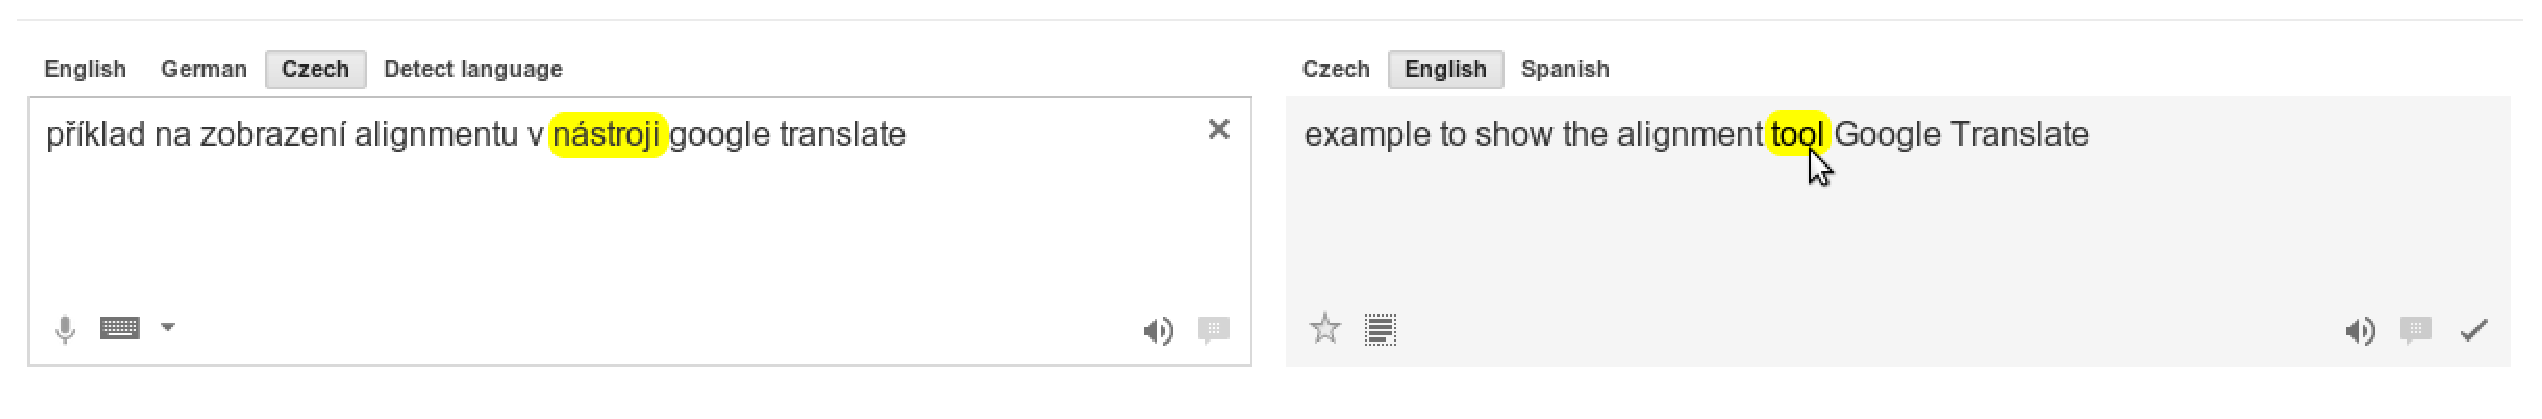
\includegraphics[width=0.9\textwidth]{img/alignment.eps}
	\caption{Ukázka zobrazení aligmentu v překladači Google Translate}
	\label{img:alignment}
\end{figure}

\section{Podobné aplikace}
Vývoj nástroje MT-ComparEval byl v určitých oblastech inspirován nástroji,
  které už mohou vývojáři běžně využívat při své práci.
Z těchto nástrojů byly vybrány nejdůležitější vlastnosti,
  které byly později zkombinovány do jednoho funkčního celku.
V následující části budou tyto nástroje podrobněji představeny.

\subsection{mteval-11b.pl}
Je skript napsaný v jazyce Perl,
  který umožňuje počítat metriky BLEU a NIST.
Tento skript je celosvětově používaný,
  a proto byl použit pro kontrolu,
  že metriku BLEU v MT-ComparEval počítáme správně.

V současné době už existuje verze mteval-13a.pl,
  v které mimojiné přibyla možnost počítat metriky pro jednotlivé segmenty v překladu.

\subsection{iBLEU}
Nástroj iBLEU umožňuje vyhodnocovat a porovnávat strojové překlady.
Pokud uživatel nemá žadný jiný strojový překlad,
  s kterým by chtěl svůj překlad porovnat,
  může si větu nechat přeložit překladačem Google Translate\footnote{
    Bohužel Google Translate nenabízí bezplatné api.
  } nebo Bing Translator\footnote{
    Bing Translator nabízí bezplatné api do limitu 2 miliónů přeložených znaků za den.
  }
  a porovnat svůj překlad s překladem z tohoto nástroje.

Pomocí tohoto nástroje můžeme počítat BLEU pro celé dokumenty nebo i jednotlivé segmenty
  a podle jejich výsledku si je můžeme později prohléhnout.

Pokud uživatel porovnává svůj strojový překlad pouze s referenčním překladem,
  je zvýrazněn jejich diff.
V případě, že uživatel porovnává dva strojové překlady,
  je zobrazen diff těchto překladů.

Tento nástroj je možné používat lokálně jako webovou aplikaci bez použití webového serveru,
  protože je celý napsán v HTML 5, CSS a javascriptu.
Stejně jako MT-ComparEval i iBLEU používá pro počítání BLEU jako referenční implementaci mteval-13a.pl.

Na Obrázku \ref{img:ibleu} je možné vidět porování dvou překladů v nástroji iBLEU.
\begin{figure}
  \center
  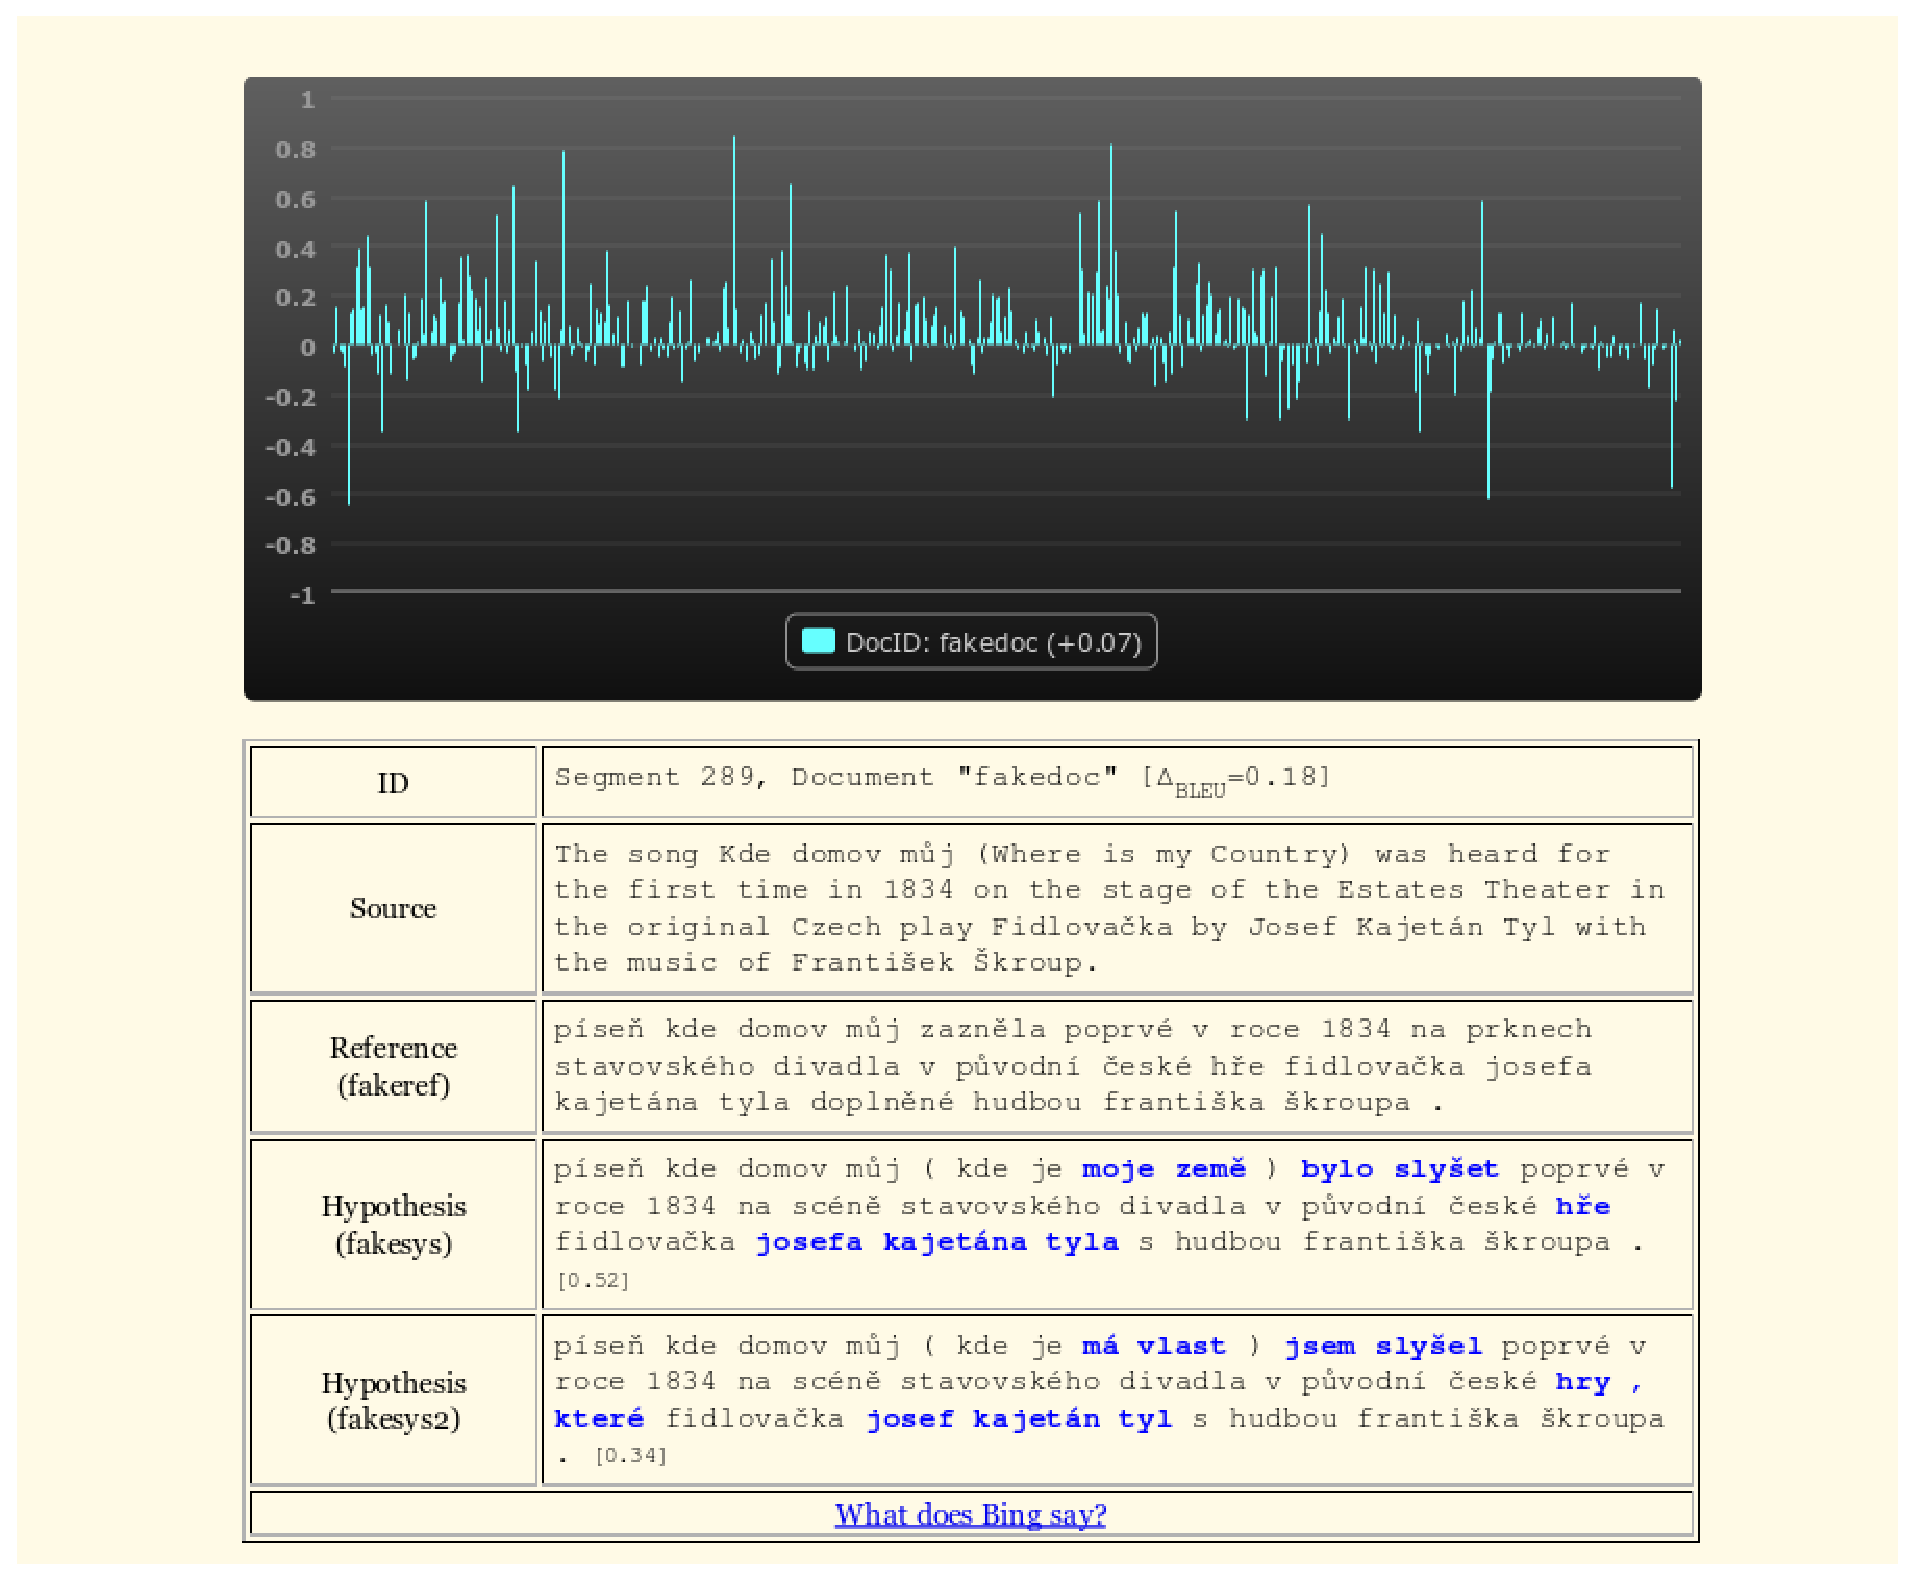
\includegraphics[width=0.9\textwidth]{img/ibleu.eps}
  \caption{Porovnání dvou překladů v nástroji iBLEU}
  \label{img:ibleu}
\end{figure}


\subsection{EMS - An Experimental Management System}
Nástroj EMS,
  který je součástí strojového překladače Moses,
  obsahuje webovou aplikaci,
  díky níž je možné porovnávat překlady.
V porovnávaných větách barevně zvýrazňuje slova,
  na základě délky nejdelšího n-gramu,
  do kterého zvýrazňované slovo patří.
Obrázek \ref{img:ems-sentence} ukazuje takto zvýrazněnou větu.
Pro n-gramy také počítá precision a recall.

\begin{figure}
  \caption{Zvýrazněné n-gramy podle délky v nástroji EMS}
  \label{img:ems-sentence}
\end{figure}

Ve webovém prostředí je též možné vyhledávat věty,
  ve kterých byl použit n-gram.
Jednotlivá užití n-gramů jsou pak rozřazena do skupin podle správnosti překladu.
Na Obrázku \ref{img:ems-word} je možné vidět seznam vět,
  ve kterých bylo použito slovo ??.

\begin{figure}
  \caption{Výpis vět, ve kterých se vyskytuje slovo ??, v nástroji EMS}
  \label{img:ems-word}
\end{figure}

Další věcí, kterou můžeme použít při porovnávání dvou překladů,
  jsou grafy správně přeložených vs. špatně přeložených slov.
Takové grafy je možné vidět na Obrázku \ref{img:ems-charts}.

\begin{figure}
  \caption{Grafy správně přeložených vs. špatně přeložených slov v nástroji EMS}
  \label{img:ems-charts}
\end{figure}

Webové prostředí nástroje EMS nabízí i další možnosti porovnání překladů,
  o kterých je možné se více dozvědět v dokumentaci tohoto nástroje.

\section{Problémy při řešení}
Při vývoji nástroje MT-ComparEval jsem narazil na mnoho problémů.
Ať už se jednalo o volbu jazyka, frameworku či databáze.

Z počátku byl nástroj MT-ComparEval vyvíjen v jazyce Perl,
  ale po několika neúspěšných pokusech byl nahrazen za jazyk PHP,
  ve kterém jsem více zběhlý.
Jelikož většina nástrojů pro strojový překlad je vyvíjena v jazyce Perl,
  nelze mu připisovat žádné mínusové body.
Chyba byla v tomto případě na mé straně.

Aby bylo možné snadno nainstalovat nástroj MT-ComparEval na vývojářově počítači,
  byla jako databáze zvolena databáze SQLite 3.
Ta vyhovuje většině požadavků.
Bohužel jsem strávil hodně času s odhalováním chyb,
  způsobených tím,
  že SQLite 3 zamyká zvláštním způsobem datový soubor,
  a proto není možné používat databázi v různých procesech.
Při normálním použití na webu se s touto chybou nepotkáme,
  protože procesy databázi používají pouze během zpracování HTTP požadavku.
Avšak při použití dlouho trvajících procesů pro import experimentů a tasků
  vždy docházelo ke kolizím při přístupu k databázi,
  které vyústili v pád importu.
Proto musel být návrh importu zcela přepracován a nyní by měl fungovat podle představ.


V duchu TDD\footnote{Test-Driven-Development}
  jsem se snažil před vlastní implementací napsat testy pomocí nástroje Behat.\footnote{http://www.behat.org}
Ten slouží k BDD\footnote{Behaviour-Driven-Development}.
Pro všechny kroky importů byly napsáný specifikace chování, které byly nástrojem Behat otestovány.
Ovšem později se ukázalo, že tento přístup k testování nebyl úplně vhodný, a testy pomocí tohoto nástroje jsem přestal psát.
Vše bylo způsobeno tím, že byla porušena pyramida testů\footnote{http://martinfowler.com/bliki/TestPyramid.html},
  jelikož všechny testy odpovídali funkčním testům.
Lepší přístup by byl vytvořit pro všechny funkční požadavky unit testy,
  jejichž spuštění by trvalo kratší dobu.


%%% Seznam použité literatury
\include{literatura}

%%% Tabulky v bakalářské práci, existují-li.
\chapwithtoc{Seznam tabulek}

%%% Použité zkratky v bakalářské práci, existují-li, včetně jejich vysvětlení.
\chapwithtoc{Seznam použitých zkratek}

%%% Přílohy k bakalářské práci, existují-li (různé dodatky jako výpisy programů,
%%% diagramy apod.). Každá příloha musí být alespoň jednou odkazována z vlastního
%%% textu práce. Přílohy se číslují.
\chapwithtoc{Přílohy}

\openright
\end{document}
